%----------------------------------------------------------------------------------------
%	PACKAGES AND DOCUMENT CONFIGURATIONS
%----------------------------------------------------------------------------------------

\documentclass[
	letterpaper, % Paper size, specify a4paper (A4) or letterpaper (US letter)
	10pt, % Default font size, specify 10pt, 11pt or 12pt
]{class}

\usepackage{caption}
\usepackage{soul}
\usepackage{subcaption}

\addbibresource{bibliography.bib} % Bibliography file (located in the same folder as the template)

%----------------------------------------------------------------------------------------
%	REPORT INFORMATION
%----------------------------------------------------------------------------------------

\title{Airline Departure\\Data Analysis and Regression} % Report title

\author{Lucchi Manuele \& Tricella Davide} % Author name(s), add additional authors like: '\& James \textsc{Smith}'

\date{\today} % Date of the report

%----------------------------------------------------------------------------------------

\begin{document}

\maketitle % Insert the title, author and date using the information specified above

\begin{center}
    \begin{tabular}{l r}
        Instructors: Professor \textsc{Cesa-Bianchi} \& Professor \textsc{Malchiodi}
    \end{tabular}
\end{center}

%----------------------------------------------------------------------------------------
%	DECLARATION
%----------------------------------------------------------------------------------------

\textit{We declare that this material,
    which we now submit for assessment, is entirely our own work and has not been
    taken from the work of others, save and to the extent that such work has been cited and
    acknowledged within the text of our work. We understand that plagiarism, collusion,
    and copying are grave and serious offences in the university and accept the penalties that
    would be imposed should I engage in plagiarism, collusion or copying. This assignment,
    or any part of it, has not been previously submitted by us or any other person for
    assessment on this or any other course of study.}

%----------------------------------------------------------------------------------------
%	ABSTRACT
%----------------------------------------------------------------------------------------

\begin{abstract}
    The purpose of this paper is to evaluate the usage of a Logistic Regression model on a airlines dataset to predict flight cancellation or diversion, in a scalable and time/space efficient implementation.
\end{abstract}

%----------------------------------------------------------------------------------------
%	TOC
%----------------------------------------------------------------------------------------

\tableofcontents

%----------------------------------------------------------------------------------------
%	DEFINITIONS
%----------------------------------------------------------------------------------------

\section{Definitions}\label{definitions} % Labels provide a point for referencing, in this case with \ref{definitions} to refer to this subsection number

\begin{description}
    \item[Dataset] The sample of data used to train the Model
    \item[Label] The expected outcome of the prediction
    \item[Model] The group of algorithms that tries to solve the problem
    \item[Overfitting] When the model is too sensible to changes compared to the dataset
    \item[Vanishing Gradient] When the gradient values becomes progressively smaller until they are insignificant for the process
\end{description}

%----------------------------------------------------------------------------------------
%	INTRODUCTION
%----------------------------------------------------------------------------------------

\section{Introduction}

The following text details an analysis on the performances of a regression model on a flights dataset, both in a time/resources usage perspective and in the outcome's precision one.\\
The computation will make use of Pyspark, a famous Python library for data manipulation on distributed environments, to test various distributed computation techniques and compare it to a serial approach.
The model will instead compare the Logistic Regression model proposed with some state of the art implementations and even different approaches.

The document is structured in a describing part, where the operations on the dataset and how the model is built are detailed and an experimental part where a series of tests are performed and the results are stated.\\

Also, the document covers two different objectives, the classification of the dataset using the model to predict both the \textbf{canceled} and the \textbf{diverted} flights.\\
The two objectives are virtually the same, since the subset of the dataset used is identical and the model stays the same, so we could expect similar results.\\


%----------------------------------------------------------------------------------------
%	DATASET
%----------------------------------------------------------------------------------------

\section{Dataset}

The initial dataset, "Airline Delay and Cancellation Data" \cite{dataset} is made of 9 years of airlines flights data, composed by 10 files (one for each year from 2009 to 2018) with around 6 milions records each.
The files presents 28 columns, of which only the 9 more relevant were took\\

\begin{description}
    \item[FL\_DATE] The flight date.
    \item[OP\_CARRIER] The carrier code.
    \item[ORIGIN] The departure airport.
    \item[DEST] The destination airport.
    \item[CRS\_DEP\_TIME] The planned departure time.
    \item[CRS\_ARR\_TIME] The planned arrival time.
    \item[CANCELLED] If the flight has been canceled.
    \item[DIVERTED] If the flight has been diverted.
    \item[CRS\_ELAPSED\_TIME] The planned total time of the flight, taxi time included.
    \item[DISTANCE] The distance the flight has to cover.\\
\end{description}

The majority of columns have been excluded because contained information not available at departure time, like the ones regarding actual departure, flight and arrival time, which are at disposal only after the aircraft landed.
Other columns also contained informations which do not have any correlation with the objective of the experiments, like the flight number assigned by the carrier.\\

In the case the prediction is about the cancellation, the \texttt{DIVERTED} column will be ignored, while if the prediction is on if the flight would be diverted or not, the \texttt{CANCELLED} column will be ignored.\\

The carrier code is a two characters alphanumeric code, the origin and destination places are a three characters alphanumeric code.\\
Flight date, departure time and arrival time are dates, while the elapsed time and the distance are real numbers.\\
Cancelled and diverted are either 0 or 1.\\

100,000 records sampled with an uniform distributed were took from each year file to perform the preprocessing. This number is due to the limited memory
possessed by the machine on which the tests have been performed.

%----------------------------------------------------------------------------------------
%	PREPROCESSING
%----------------------------------------------------------------------------------------

\section{Preprocessing Techniques}

\subsection{Null values removal}

Multiple preprocessing techniques were used.\\

The first operation consisted in the removal of the rows with null values, after counting them the conclusion was that the null values are really rare in the dataset, so it was possible to remove the rows entirely, without any significant loss of informations.\\

\subsection{Data Analysis}
After the null rows removal, some analysis have been performed using the charts of the MatPlotLib library, especially the bar charts.\\
The main objective of this analysis was to find an eventual relationship between the various features used and the probability that a flight would be cancelled or diverted.\\

None of the features showed significative patterns nor tendencies of the problematic flights to increase in relation to a particular value of a feature or a combination of features both the analysis of the dataset and the actual model costruction, probably because the dataset doesn't include informations on events that usually leads to this outcomes.\\

\subsubsection{Problematic flights per carrier}
The first chart drawn tried to correlate the carriers with an abnormal number of the cancelled flights, to make the chart more readable, every carrier with a percentage lower than the mean of all carriers was aggregated into a single column, to show only the highest percentages.\\

The result was a chart showing some carriers with a slightly-above-average number of cancelled flights, and a peak of 4\% of the flights  cancelled, but considering the huge number of distinct carriers in the dataset, the impact of this feature will probably be very low.

\begin{center}
    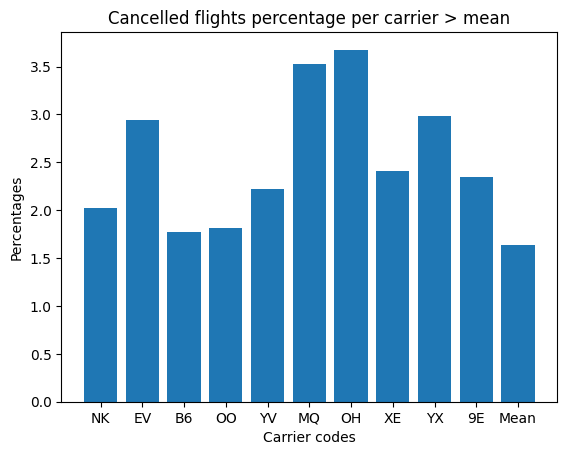
\includegraphics[width=10cm]{../images/cancelled_per_carrier.png}
    \captionof{figure}{}
\end{center}

\subsubsection{Problematics flights per origin}
The second analysis was performed on the origin feature.
The first chart plotted was a box plot, because due to the high number of airports, the bar was overcrowded and diffcult to read.\\

The result can be considered an improvement regarding the correlation between a feature and the result, because thre are some origins that posses a significant percentage
of problematic flights, with a peak of over 25\% of cancelled flights. This cannot be taken as a decisive factor though, because while the probability of those particular airports increase notably, the vast majority of the origins (at least two quartiles), show no evident correlation with this feature.

\begin{center}
    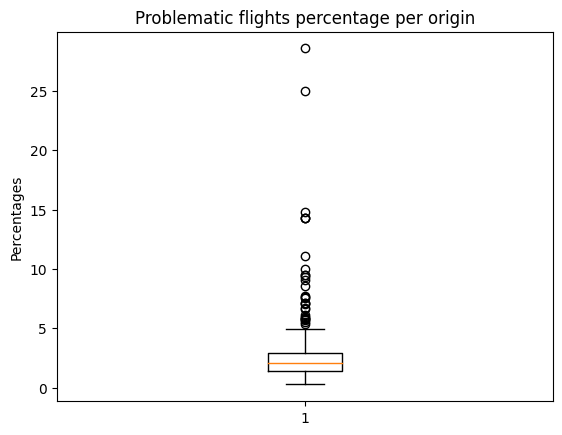
\includegraphics[width=9cm]{../images/cancelled_box_per_origin.png}
    \captionof{figure}{}
\end{center}

To show a readable bar chart, a similar technique as before has been applied, the chart shows only the airports where there is a rate of cancelled flights above 5\%. This time it was not enough to remove the bars below the mean of the values, so a fixed number was used to filter the showing bars, which is switched based on the problem to solve,
because the diverted problem possesses lower percentages of problematic flights.

\begin{center}
    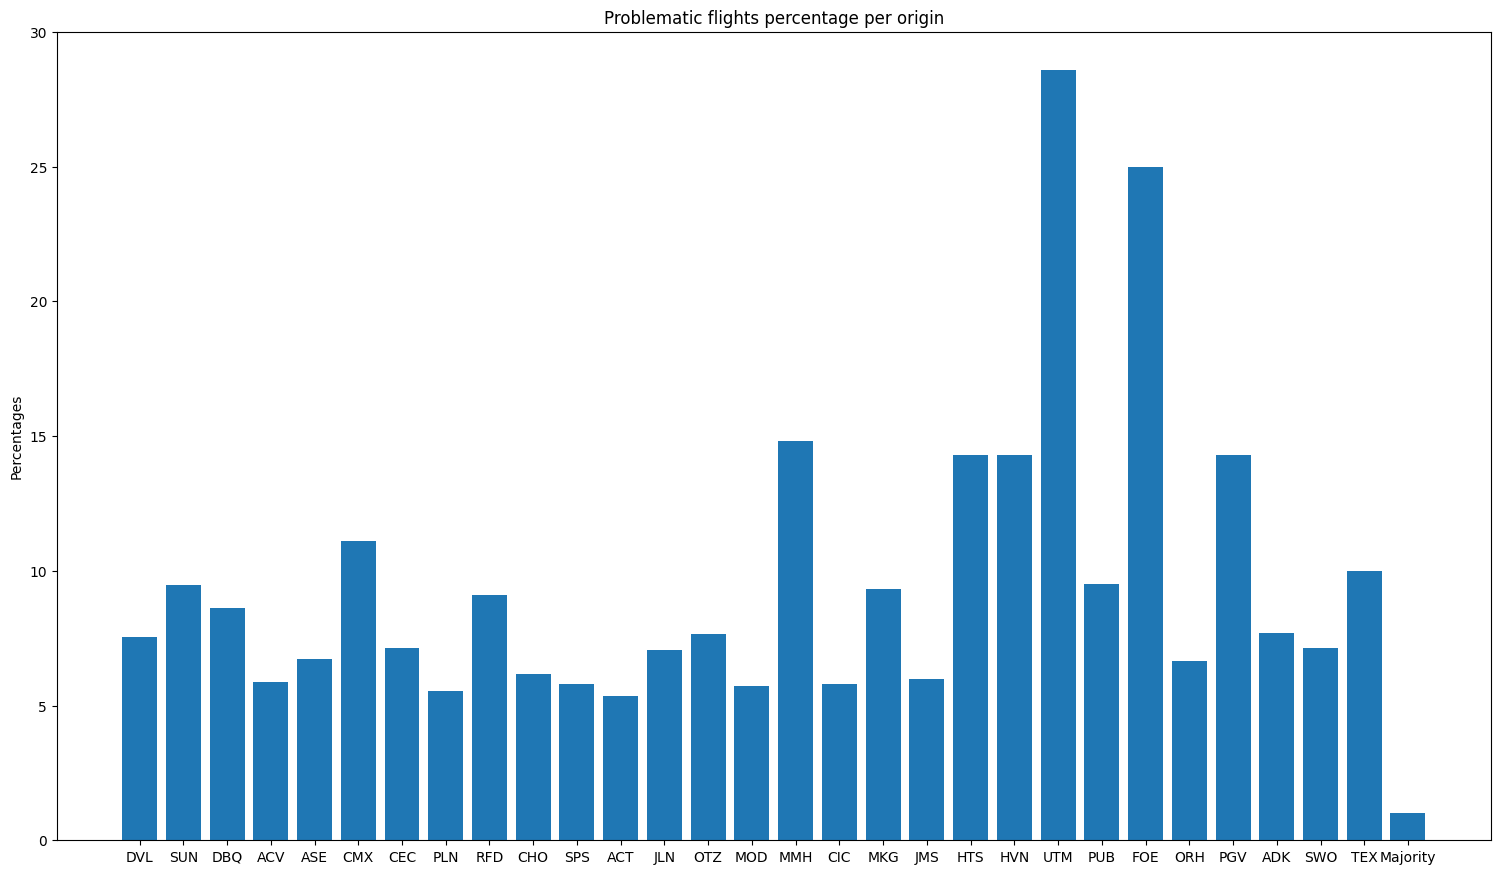
\includegraphics[width=14cm]{../images/cancelled_per_origin.png}
    \captionof{figure}{}
\end{center}
\newpage

\subsubsection{Problematics flights per month}
Trying to find a correlation between the year period and the problematic flights, a chart based on the month of the flight has been plotted. The result was expectedly skewed towards the winter months, where the bad weather conditions can influence the flight departures, but even in this case, the difference was not so dramatic, always remaining in a few percentage points.

\begin{center}
    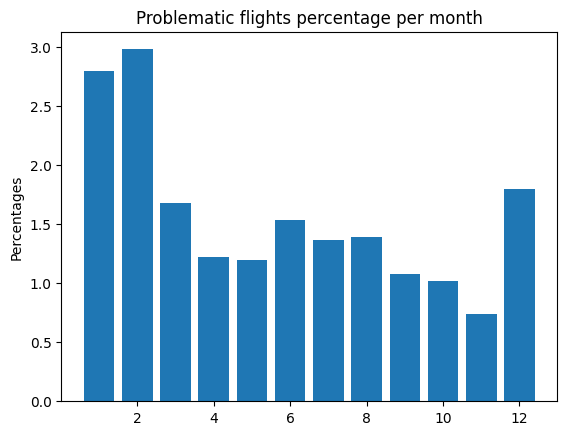
\includegraphics[width=10cm]{../images/cancelled_per_month.png}
    \captionof{figure}{}
\end{center}

\subsubsection{Problematics flights per weekday}

The last chart was based on the weekday of the flight, trying to see if there was a relation between particular days and the rise of problematic flights.\\

Unfortunately this was the most useless analysys performed, with every column of the chart being almost identical to each other, basically this information doesn't tell anything about the probability of a flight of being problematic or regular.

\begin{center}
    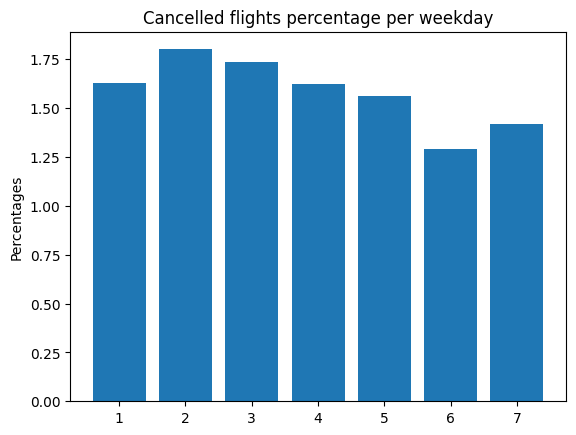
\includegraphics[width=10cm]{../images/cancelled_per_weekday.png}
    \captionof{figure}{}
\end{center}

\subsection{Data conversions}

All the data not already represented as real numbers have been converted; airports and carriers identifiers, that were alphanumeric codes, had a number assigned based on the code. Dates were splitted between the year and the rest, the former has been discarded, while the latter has been hashed.\\

\subsubsection{Hashing}

Particularly, to convert the identifiers, the checksum function \textbf{crc32} \cite{crc32} has been used, then the result has been put in END with the bytes representing the number -1, to ensure to get an unsigned integer. Finally, the value is normalized dividing it for the max integer value.
This function has been chosen because is one of the fastest way to hash short strings, which is what is needed here, compared to other alghoritims like the SHA or MD5.\\

\subsubsection{Normalization}

To normalize dates, the day of the year has been extracted from every date, then divided by 365. A similar strategy has been used for the departure and arrival times, exctracting the minutes of the day and then dividing by 1140.\\

The distance has been normalized by dividing it for the maximum value found in the dataset, rounded by excess to 4970.\\

At this point, the dataset has been balanced in regard of the evaluated property, be it being canceled or diverted, so that there are an equal number of uniformly drawn positives and negatives.\\

The converted values were also limited between 0 and 1, to avoid exploding values during the training of the model.\\

\subsubsection{Balancing}

This was necessary since the diverted or cancelled flights are a really small percentage of the overall flights,
this in the first tests has been proved to be a problem, because the trained model always responded that no flight would have been cancelled or diverted, since it has been trained on a dataset with basically zero problematic flights.\\

To solve the problem, the \textbf{Undersampling} technique has been used, matching the number of normal flights and problematic flights, limiting the amount of normal flights that has been kept.\\

Since less than 0.1\% of the dataset are positive cases (for both the tasks) after the oversampling, the records remained are just some tens of thousands, instead of hundreds of thousands, half with positive outcomes and half with negative ones.\\

The following charts show the \texttt{REGULAR} and \texttt{CANCELLED} flights before and after balancing:\\

\begin{figure}[!htb]
    \centering
    \minipage{0.5\textwidth}
    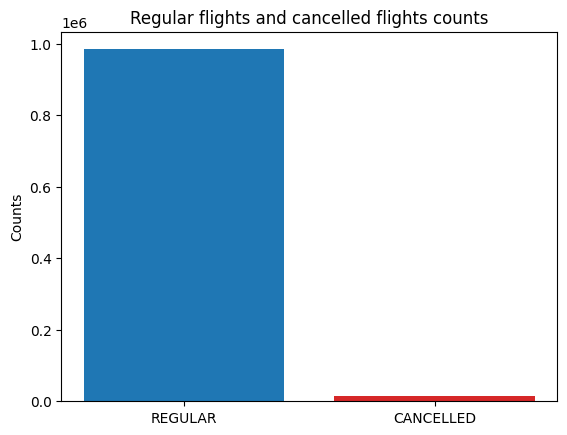
\includegraphics[width=\linewidth]{../images/cancelled_unbalanced.png}
    \endminipage\hfill
    \minipage{0.5\textwidth}
    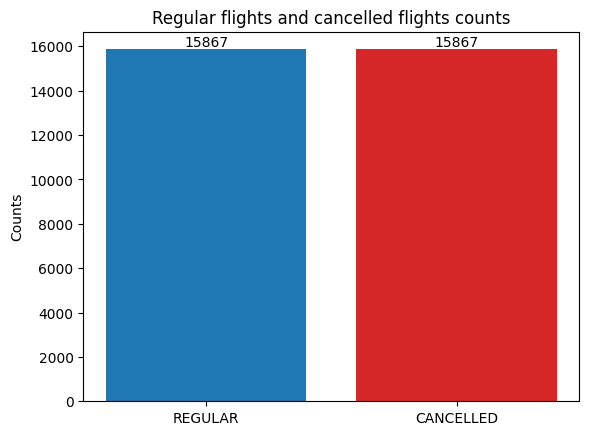
\includegraphics[width=\linewidth]{../images/cancelled_balanced.png}
    \endminipage\hfill
    \captionof{figure}{}
\end{figure}

\subsubsection{Z-Score Normalization}
Before the actual computation, the dataset has been normalized again by subtracting the \textbf{mean} and dividing by the \textbf{standard deviation}. This is called \textbf{Standard Score} \cite{normalization} or Z-Score Normalization.\\

The purpose of this normalization is to present to the model data that possesses less noise, improving the training performance. Particularly in this scenario, where the model proposed is simple and not sophisticated enough to work well with data that are not normalized.

\subsubsection{K Fold Cross Validation}
After the dataset has been processed, the resulting data must be splitted into a \textbf{training} part and a \textbf{testing} part. To avoid bias towards specific parts of the dataset, the K-Fold Cross Validation \cite{crossvalidation} was used.\\

This technique consists on splitting the dataset into K equally distributed and sized parts called folds, and while K-1 folds will be used for the training, the other one will be used for testing. This process will be repeated for K time, using each time a differend fold for the testing (and consequently excluding it from the training)\\

During the split, the percentages of positives and negatives cases have been kept costant for every partition, it has been ensured that every fold has a different set of rows to avoid overlapping of any kind.

$$ x' = \frac{x - \mu}{\sigma} $$

\subsection{Parallelization}

\subsubsection{PySpark}
Keeping in mind that the implementation has to be space and time efficient and \textbf{scale up to large datasets}, the preprocessing part has been carried out using the library PySpark.
PySpark is a wrapper for Python of the library Apache Spark \cite{spark}, originally written in Java.\\

The purpose of this library is the handling of \textbf{parallelized data processing}, particularly regarding the Distributed File System Hadoop, also created by the Apache Foundation.
The library handles automatically the work distribution on the available nodes that the system provide, it can be composed of a single machine with multiple cores or a cluster of machines, this improves significantly the \textbf{scalability} of the solution, which can be run on competely different system without code modification.\\

\subsubsection{Compatibility}

The usage of this library created some compatibility issues, because the data structures used by PySpark were not compatible with various parts of the preprocessing section, which had been written initially using the data science library Pandas \cite{pandas}.\\

To solve these problems, it wasn't possible to simply use a conversion and leave the parts written in Pandas as they were, because the computation would have run on a single machine, without parallelization, making the use of PySpark completely pointless.
The issue has been addressed using the \textbf{PySpark.SQL} functionality, which allow to execute queries on a distributed dataframe. For our purposes various UDF (User Defined Functions), have been created, which then have been applied to every column containing certain types of data.
When it was possible, the conversions have been accomplished using a select method only, because the UDF functions are not as optimized as the native ones, making the computations with UDF significantly longer.\\

To evaluate the differences between the PySpark and Pandas performances, the preprocessing part has been implemented using both methods, with the possibility to test the Pandas implementation in its own code cell.

\subsubsection{I/O}

The library PySpark is also able to handle the csv file reading and writing, so it has been used to save the preprocessed data to speed up multiple runs on the dataset. To carry out the writing of the various distributed dataframes, various files are created, then at the time of reading, the data is distributed to the various nodes. There are two intermediate csv files, one for the 'cancelled' problem and one for the 'diverted' problem.\\

\subsubsection{Data structures}

The preprocessing part of the solution uses the PySpark \textbf{Dataframe} structure, the main reason for this choice is to take advantage of the column notation. This makes the code cleaner and easier to read, than the standard RDD (Resilient Distributed Dataset) implementation. The dataframe SQL functions are also really handy to convert efficienlty the various columns of the dataframes.
However, after the preprocessing, entering the training section of the project, it looked like the RDD structure was better suited to accomplish the various calculations required by the model, so the folded dataframes were converted to RDDs before passing them to the next section.

\subsubsection{Caching}

The \textbf{cache} method has proven to be a fundamental piece to improve PySpark computation performances. This method saves in the main memory the reuslts of the transormations applied to a dataframe at the moment when its called. Caching after the data loading brought a significant reduction in computation time. Before the using of this method, folding part was almost unviable due to the huge amount of time required by the procedure.
This method was also used in the parallel training part, by caching the various batches to process.


%----------------------------------------------------------------------------------------
%	MODEL
%----------------------------------------------------------------------------------------

\section{Model}

The proposed model is a simple Logistic Regression \cite{logistic} algorithm that makes use of a few techniques to avoid overfitting (batching, L2 regularization) and uses the Gradient Descent as a solver.\\
The implementation uses \textbf{numpy} \cite{numpy} as its primary library of mathematical functions

\subsection{Parameters initialization}
Parameters such as Weights and Bias are initialized using a \textbf{uniform distribution} between 0 and 1, with the first one having the same length as the number of columns and the second being a scalar value.
The other hyperparameters were tuned throught various experiments that will be detailed later.

\subsection{Algorithm}

\subsubsection{Estimate}
The estimate is computed as follows
$$ \hat{y} = \sigma(w^Tx + b) $$
where $\sigma$ is the Sigmoid function \cite{sigmoid} and it's defined as
$$ \sigma(z) = \frac{1}{1 + e^{-z}} \in [0,1] $$
and $w$ and $b$ are the model weights and bias and $x$ is the input.

The code implementation uses \texttt{np.exp} for the exponential calculation.

\subsubsection{Gradient}

$$ \nabla w = \frac{1}{m}x^T(\hat{y} - y) $$
$$ \nabla b = \frac{1}{m}\sum(\hat{y} - y) b $$

In the code implementation, \texttt{np.dot} and \texttt{np.mean} were used.

\subsubsection{Update}

Gradient Descent \cite{sgd} is a technique that allows to find maximus e minimum in a multi-variable function, like the model taken in consideration.\\
Once the gradients are calculated, the parameters (weights and bias in this case) will be updated with the gradient value properly mitigated with the \textbf{Learning Rate}

$$ w' = w - \mu \nabla w $$
$$ b' = b - \mu \nabla b $$

\subsubsection{Loss}
For the loss the \textbf{Binary Cross Entropy} \cite{binarycrossentropy} function, also called \textbf{Log Loss}, was used.
It is defined as
$$ loss(\hat{y}, y) = -\frac{1}{n}(y log(\hat{y}) + (1-y)log(1-\hat{y})) $$
This particular function is used since, to perform the gradient descent, it can be derived and conducted to the weights update formula to minimize the loss in the same way as it's done for the MSE \cite{mse} in the Linear Regression.\\

For the MSE and Linear Regression

$$ MSE(w) = \frac{1}{2} (\hat{y} - y)^2 = \frac{1}{2} (w^Tx - y)^2 $$
$$\frac{\partial J}{\partial w} = (w^T x - y)x $$
$$ w' = w - \mu (w^T x -y)x $$

For the Log Loss and Logistic Regression

$$ LogLoss(\hat{y}, y) = -y log \hat{y} - (1-y)log(1- \hat{y})$$
$$ \hat{y} = sigmoid(w^Tx) = \frac{1}{1 + e^{w^Tx}} $$
$$ \frac{\partial LogLoss}{\partial w} = (\hat{y} - y)x $$
$$ w' = w - \mu (\hat{y} - y)x $$
$$ w' = w - \mu (w^T x -y)x $$

\subsubsection{Batching}
There are multiple types of Gradient Descent.\\

\textbf{Stochastic Gradient Descent} updates the model after each sample and has a convergence rate that is non-linear $O(\frac{1}{k})$ where $k$ is a fixed step size.\\

\textbf{Batching Gradient Descent} updates the model once per iteration using the whole dataset at once. It has a better convergence rate.\\

\textbf{Mini Batch Gradient Descent} \cite{batching} uses small chunks of samples, so it's a middle solution between the previous ones, but adds a new hyperparameter to tune, the \textbf{Batch Size}.\\
Its convergence rate is
$$O(\frac{1}{\sqrt{bk}} + \frac{1}{k})$$

In this project the last one was choosen after a dedicated experiment.

\subsubsection{Regularization}
Regularization is a technique used to prevent the overfittings. A regularization term is added to the optimization problem (i.e. the gradient calculation) to avoid overfitting.
The used version is called \textbf{L2}, also known as \textbf{Ridge Regression} \cite{l2}.\\

The regularization factor for the loss is defined as
$$ L2 = \frac{\lambda}{2}||w||^2 $$
where $L2$ is calculated as
$$ \frac{\lambda}{2}||w||^2 = \frac{\lambda}2{\displaystyle\sum_{j=1}^m w_j^2} $$ \\

The loss then becomes
$$ loss(\hat{y}, y) = -\frac{1}{n}(y log(\hat{y}) + (1-y)log(1-\hat{y})) + \boldsymbol{\frac{\lambda}{2}||w||^2} $$

While the weights gradients formula becomes
$$ \nabla w = \frac{1}{m}x^T(\hat{y} - y) \boldsymbol{+ \lambda w} $$

\subsubsection{Hyperparameters}
To train a model, some parameters complementary to the dataset that influence the training should be individuated and their values tuned to try to find the global minimum of the function the user is trying to reproduce.\\
In this case, there are 3 parameters:
\begin{enumerate}
    \item The number of iterations
    \item The Learning Rate
    \item The constant for the L2 Regulation
\end{enumerate}

\subsubsection{Model Implementation}
As stated before, the parallel version of the model has been implemented using RDDs and the MapReduce paradigm. This is since SQL syntax is not suited for mathematical operations and at this stage of the execution, all the data has been converted to float, so there is no need for the DataFrame schema anymore.\\
The MapReduce paradigm is the perfect way to parallelize bitwise operations followed by a reduction, like the dot product. And since most of the operations in training a machine learning model are matrix multiplications, that are a sequence of dot products, there should be a gain in performances.

\subsection{Differences with Pyspark ML and Sklearn implementation}

In the following chapters the presented model performances will be compared with the Sklearn implementation \cite{logisticsklearn}, that has quite some differences.\\
First, both the Pyspark and the Sklearn version doesn't use the SGD solver, where the first one doesn't appear to specify what approach it uses and the second one uses \textbf{L-BFGS-B - Software for Large-scale Bound-constrained Optimization} \cite{lbfgsb}, by default.
In both case the solver doesn't need any form of Learning Rate.\\
Also, with these implementations, the L2 Regularization is enabled by default as well.

\subsection{Differences with other algorithms: Decision Tree}
The Decision tree is a predictive model where each node represents a variable, each arc is a possible value for that property and each leaf is the predicted value for that variable based on the values of the other properties.\\
To compare the previous results to a Decision Tree Classifier, the Pyspark ML implementation has been used. This version supports both binary and multiclass classification, as well as both continuous and categorical features.\\
Due to the structure of the problem, only the binary classification is needed. Also, since the dataset is already converted from categorical to continuous data, there's no need for other conversions.\\
Similarly to the Logistic Regression library from Pyspark, the model accepts directly a parallel DataFrame.

%----------------------------------------------------------------------------------------
%	EXPERIMENTS
%----------------------------------------------------------------------------------------

\section{Experiments}

The first wave of experiments follows the performances and results of the techniques described and implemented in this research.

\subsection{Test Hardware}

To perform the experiments, two environments were setupped.
\begin{enumerate}
    \item A powerful and multicore execution context, represented by device with a last generation 8 core and 16 thread Ryzen CPU with 16GB of RAM and an high speed SSD, which the following results are based on.
    \item A more accessible cloud environment represented by a Google Colab base instance, with a dual core virtual CPU and 12 GB of RAM
\end{enumerate}

\subsection{Preprocessing Performance}
\subsubsection{Time}
The table below summarizes the time required to complete various parts of the preprocessing section.\\
All this tests have been performed on the same machine to avoid differences due to hardware performances.

In order to collect the data of PySpark, at the end of every section the method count() was launched, forcing the library to execute immediately the operation requested.\\

Without these requests, the lazy behaviour of PySpark data structures makes any type of benchmarking impossible.This probably makes the times of execution longer, due to
the execution of the count operations, and the \textbf{loss of some optimization} thath could be done if the library evaluates all the operations in one run.
This delay must be taken into consideration, but should not alter the overall results of the tests.\\

The numbers represents seconds of execution.

\begin{center}
    \begin{tabular}{ |c|c|c|c|c|c| }
        \hline
        Section             & Pandas   & PySpark   \\
        \hline
        Data reading        & 95.57988 & 17.09711  \\
        Null values removal & 0.33791  & 60.71444  \\
        Balancing           & 0.09456  & 25.36964  \\
        Column conversions  & 0.42862  & 1.42960   \\
        Normalization       & 0.17330  & 64.45151  \\
        Folding             & 0.18040  & 181.06777 \\
        Total               & 96.79467 & 350.13007 \\
        \hline
    \end{tabular}
    \captionof{table}{Performance comparison between Pandas preprocessing and distributed PySpark preprocessing}
\end{center}


Due to the limitations of the hardware used during the experiments, both locally and on Google Colab, there weren't significant improvements over preprocessing speed using PySpark, because of the lack of a high number of worker nodes.\\
It's worth noticing though that Pyspark used correctly every core of the host, almost at maximum power, so the problem does not reside in the handling of the underlying hardware, the performance decrease must be caused by other factors.

The only section where there is a noticeable improvement is the data reading section, in the remaining ones the performances gets worse, even significantly worse, especially in the splitting section, where PySpark takes an enormous amount of time, to perform
an operation completed in less than one second by Pandas.\\

The differences found are not stable between the various phases of preprocessing, this seems to suggest that some operations, like the normalization or the null dropping, take a higher toll over the distributed system of PySpark,
forcing it to waste more time than others to organize the parallel computation, even if they appear as simpler processes.
This could be explained by the big overhead the distributed enviroment creates that cannot be transformed into an advantage given the inadequate hardware.\\

It's also worth noticing that the Google Colab enviroment was really unstable, with the same sequence of operations taking different times in the order of \textbf{30-40\%} of difference.
\textbf{As a result, this data does not really provide any valuable conclusion regarding the preprocessing phase analysis.}\\

This suggests that the PySpark processing procedure would gain advantage over Pandas only over a really large dataset, where the time used to put up the processing infrastructure is justified by the huge amount of data to be processed.
In this case instead, it seems that most of the time required by PySpark is wasted organizing the computation, without gaining any advantage from this organization, over a library that procedes straight up to the calculation of the results.\\

It si also possible that the time required would go down if the execution took place on a more parallelized machine than the Colab enviroment, giving PySpark the opportunity to take advantage of work distribution on a higher number of nodes.
\subsubsection{Memory}

Another interesting comparison to make is the memory usage. This analysis would be more significative if Pysaprk could use more than one machine to distribute the workload over multiple nodes, but it will be reported anyway.\\

\begin{itemize}
    \item \textbf{Pandas Memory Usage}\\
          In this case the RAM usage was stable around 1.2 GB, with some peaks.
          \begin{itemize}
              \item Average: 1.2 GB
              \item Peak: 1.6 GB
          \end{itemize}
    \item \textbf{PySpark Memory Usage}\\
          PySpark doubled the space required, with every step adding the amount indicated below to the former one.
          \begin{itemize}
              \item Dataset reading: 1 GB
              \item Null rows value dropping: 1.1 GB
              \item Dataframe balancing: 0.4 GB
              \item Columns conversion: 0.4 GB
              \item Z score normalization: 0.3 GB
              \item Splitting: 0.3 GB
          \end{itemize}
\end{itemize}


\subsection{Hyperparameter Tuning}
To choose the hyperparameters tuple $\theta$ such that the loss of the model trained using said hyperparameters is minimized, the \textbf{search grid}.
This technique consists on the choice of multiple different values for each parameter and the creation of a permutation that leaves a set of tuples with all possible combinations.\\
The model is then trained for each tuple and the losses compared, resulting on the best model the one with the lowest loss.

\begin{center}
    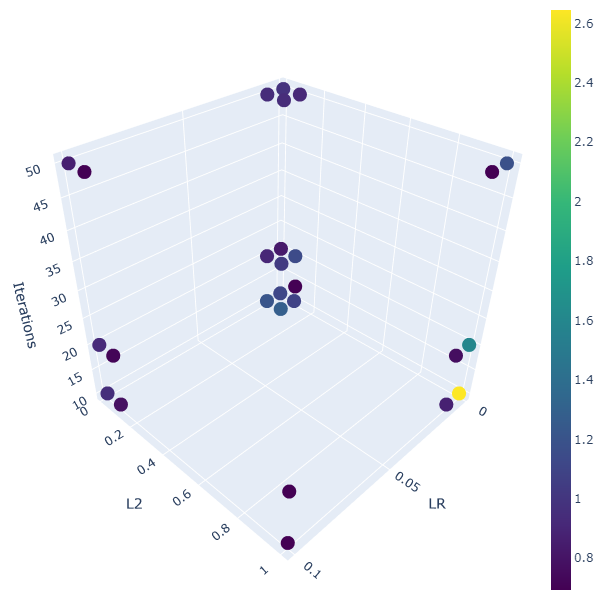
\includegraphics[width=10cm]{../images/3d.png}
    \captionof{figure}{Parameters Space for the model}
\end{center}

As can be seen in the 3D chart above, that represents the resulting losses for each different configuration of parameters (also called \textbf{hyperparameters space}), some values like a very small Learning Rate results in an high loss.\\
What follows are the values for the best configuration

\begin{center}
    \begin{tabular}{ |c|c|c|c| }
        \hline
        Iterations & LR  & L2 & Loss   \\
        \hline
        10         & 0.1 & 1  & 0.6931 \\
        \hline
    \end{tabular}
    \captionof{table}{Parallel Logistic Regression best configuration}
\end{center}

For the same configuration

\begin{center}
    \begin{tabular}{ |c|c|c|c|c|c|c|c|c|c| }
        \hline
        TN  & TP  & FN  & FP  & Precision & Recall & F1       & Accuracy & Specificity & AUROC  \\
        \hline
        789 & 800 & 762 & 773 & 0.5085    & 0.5121 & 0.510367 & 0.5086   & 0.505122    & 0.5086 \\
        \hline
    \end{tabular}
    \captionof{table}{Parallel Logistic Regression Metrics}
\end{center}

And the following ROC curve

\begin{center}
    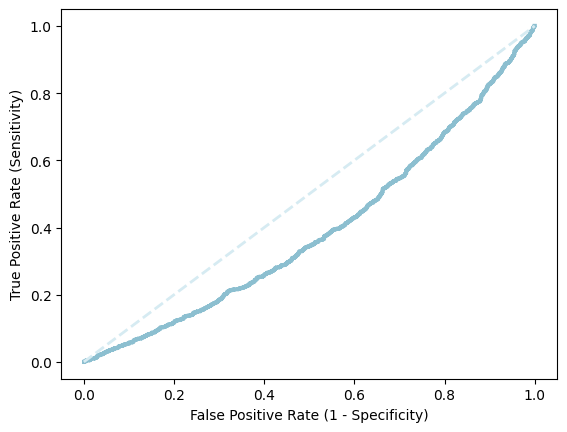
\includegraphics[width=10cm]{../images/parallel_roc.png}
    \captionof{figure}{Parallel Logistic Regression ROC}
\end{center}

It took \textbf{61 minutes} to compute all the 27 configurations, with the ones with 50 iterations taking most of the time.

\subsection{Mini Batch}

Another technique described before is the use of Mini Batches, chunk of the train datasets after each one the parameters are updated that should result in a better convergence rate.\\
However not only there wasn't any noticeable difference in the quality of the model, as can be seen in the following table

\begin{center}
    \begin{tabular}{ |c|c|c|c|c|c|c|c|c|c|c| }
        \hline
        Loss   & TN  & TP  & FN  & FP  & Precision & Recall & F1     & Accuracy & Specificity & AUROC  \\
        \hline
        0.6802 & 814 & 945 & 617 & 748 & 0.5581    & 0.6049 & 0.5806 & 0.5630   & 0.5211      & 0.5630 \\
        \hline
    \end{tabular}
    \captionof{table}{Mini Batch version of the algorithm}
\end{center}

but the performances of the parallel enviroment were greatly penalized by this different management of the datasets, resulting in processing time increased enough for it to not be completed by the available hardware.\\
This can be reconducted on the overhead added by the exchange of messages, that increases with the fragmentation of the memory and computations.
The sequential implementation has been used and it just took 2.4 seconds.

For thse reasons, the Mini Batch technique doesn't seem an option worth for this specific experiment.

\subsection{Sequential Implementation}

Since the Pyspark implementation is full of options and various optimizations, it's difficult to compare it in term of speed with the proposed implementation.\\
Thus, a sequential version with the same algorithm has been implemented. The difference is not functional but just technical, since the computation is entirely done by numpy and not also by PySpark MapReduce.

By default, numpy uses a single thread and it's optimized for sequential computation. While using a single core instead of all the available ones is tipically a disadvantage, Pyspark is built for distributed computation and for this readon it has a certain overhead.\\
This overhead resulted in a staggering difference, since the sequential implementation took about \textbf{2 minutes and 12 seconds}.

\subsection{Pyspark ML Logistic Regression}

As stated before, the proposed model has been compared to the Pyspark ML implementation of the Logistic Regression Model.
Since there's no learning rate, the hyperparameters grid is smaller, leading to less configurations to train.
Temporal wise, the computation took \textbf{37 seconds}, which is dozen of times faster than the proposed implementation even considering the fewest configurations.

The following table represents the obtained results

\begin{center}
    \begin{tabular}{ |c|c|c|c|c|c|c|c|c|c|c| }
        \hline
        Loss   & TN  & TP  & FN  & FP  & Precision & Recall & F1     & Accuracy & Specificity & AUROC  \\
        \hline
        0.6108 & 834 & 906 & 591 & 720 & 0.5571    & 0.6052 & 0.5802 & 0.5703   & 0.5366      & 0.5709 \\
        \hline
    \end{tabular}
    \captionof{table}{Pyspark ML Logistic Regression Metrics}
\end{center}

And the following ROC curve

\begin{center}
    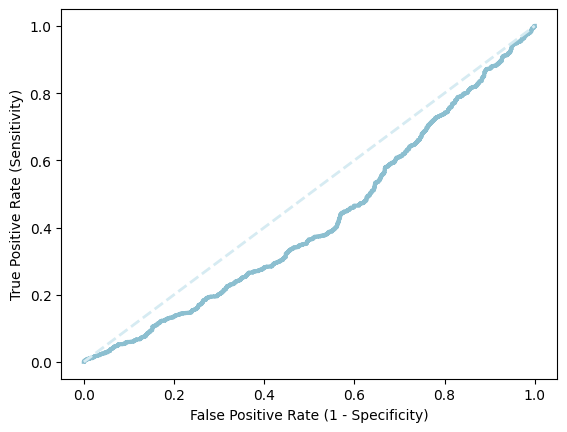
\includegraphics[width=10cm]{../images/ml_logistic.png}
    \captionof{figure}{Pyspark ML Logistic Regression ROC}
\end{center}

To compare the quality of the custom trained model and the Pyspark model, weights value can be compared. The following table shows the values of each element of the weights for each model and their absolute difference

\begin{center}
    \begin{tabular}{ |c|c|c|c|c|c|c|c|c|c|c| }
        \hline
        Custom  & Pyspark & Absolute difference \\
        \hline
        -0.0950 & -0.0823 & 0.0127              \\
        -0.0378 & 0.0445  & 0.0823              \\
        0.0233  & 0.0343  & 0.0110              \\
        -0.2209 & -0.2550 & 0.0359              \\
        0.1156  & 0.0956  & 0.02                \\
        0.0301  & -0.0072 & 0.0373              \\
        -0.1946 & -0.1940 & 0.0006              \\
        \hline
    \end{tabular}
    \captionof{table}{Comparison between models weights}
\end{center}

This comparison can also be easily done in the code using the \textbf{np.allclose}, that compares two vectors elementwise.
As can be seen the elements are close by \textbf{~0.08}, a very small value that implies similar expected results during the evaluation.\\

It's worth notice the weights absolute values are very small, meaning that for both the implementations, none of the corresponding features are impactful on the prediction.\\
It's then clear that the Logistic Regression, at least on how has been used in these experiments, \textbf{is not the correct choice for this complex problem.}\\

Besides, reaching this local minimum after just 10 iterations means that a further number would not improve the situation in any case, creating a situation were repeating the tuning multiple times could produce a different best configuration.

\subsection{Pyspark ML Decision Tree}

As stated before, another algorithm has been used to compare the proposed solution to a completely different approach.\\
The Decision Tree ended up having better results than the Logistic Regression, with a bigger Area Under the Curve.\\
What follows are the complete metrics

\begin{center}
    \begin{tabular}{ |c|c|c|c|c|c|c|c|c|c|c| }
        \hline
        Loss   & TN   & TP  & FN  & FP  & Precision & Recall & F1     & Accuracy & Specificity & AUROC  \\
        \hline
        0.5250 & 1019 & 832 & 665 & 535 & 0.6086    & 0.5557 & 0.5810 & 0.6066   & 0.6557      & 0.6057 \\
        \hline
    \end{tabular}
    \captionof{table}{Pyspark ML Decision Tree Metrics}
\end{center}

And the ROC curve

\begin{center}
    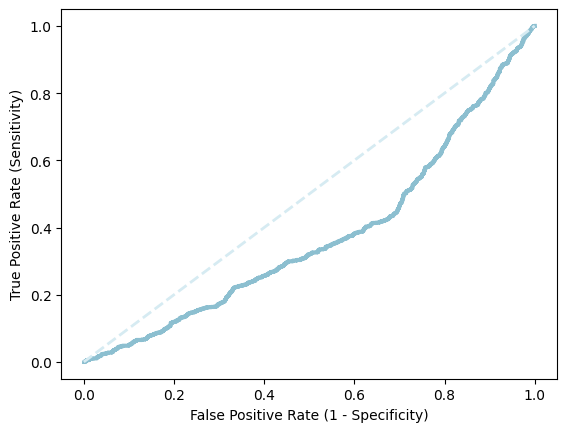
\includegraphics[width=10cm]{../images/tree_roc.png}
    \captionof{figure}{Pyspark ML Decision Tree ROC}
\end{center}

The hyperparameters grid for this experiment is smaller, with just 2 hyperparameters leading to few different configurations and it just took \textbf{7.6 seconds}.

\section{Diverted Flights}

As specified at the start of the document, all the observations and implementations have been thought to be valid for both the initial problems and considering all the previous experiments, the overall results are similar with some differences.\\

\subsection{Dataset \& Preprocessing}
The considerations on the dataset are the same, since both of the possible problems come up when there's too much delay before the start or bad climate conditions (often caused by the time of the year). In the same way, every tested aggregation didn't show any particular correlation between the data and the occourrence of the problem.\\
The feature taken and the way they are processed are therefore the same, with the only exception being the results column, changed from the cancelled one to the diverted one.\\

The only difference in this section is that the \texttt{DIVERTED} flight number is quite inferior than the \texttt{CANCELLED} one, this play a significant role in reducing the preprocessing time required.
As shown in the following balancing charts, the diverted flights are just some thousands:\\

\begin{figure}[!htb]
    \centering
    \minipage{0.5\textwidth}
    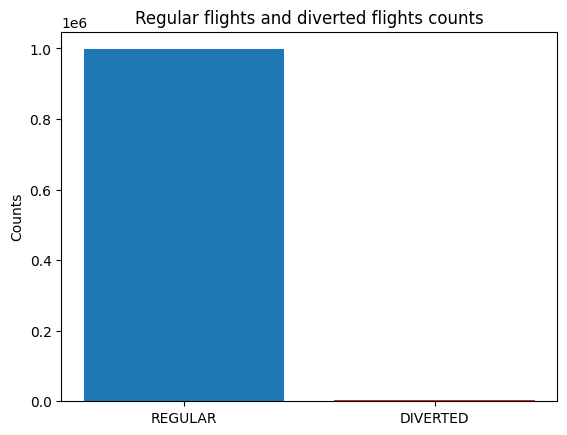
\includegraphics[width=\linewidth]{../images/diverted_unbalanced.png}
    \endminipage\hfill
    \minipage{0.5\textwidth}
    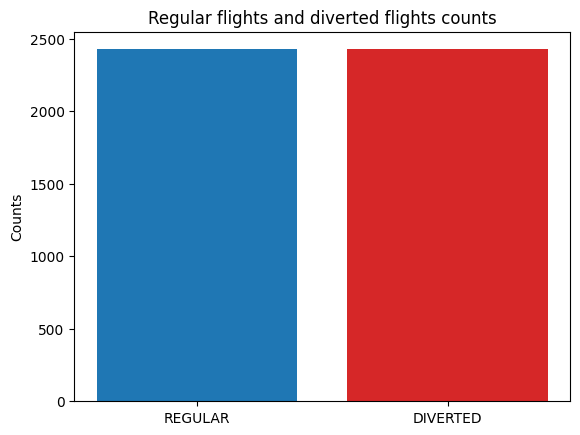
\includegraphics[width=\linewidth]{../images/diverted_balanced.png}
    \endminipage\hfill
    \captionof{figure}{}
\end{figure}

\begin{center}
    \begin{tabular}{ |c|c|c|c|c|c| }
        \hline
        Section             & Time in seconds \\
        \hline
        Data reading        & 18.5            \\
        Null values removal & 67              \\
        Balancing           & 5.5             \\
        Column conversions  & 0.4             \\
        Normalization       & 18.3            \\
        Folding             & 9.9             \\
        Total               & 119.6           \\
        \hline
    \end{tabular}
    \captionof{table}{Preprocessing performance using PySpark for \texttt{DIVERTED} flights}
\end{center}

\subsection{Model \& Training}
Since the data is still represented by the same conceptual columns represented in the same way, the model remained the same.
The execution of the experiments, starting with the hyperparameters search grid of the proposed implementation, resulted once again on a problem too complex to solve with a decent precision by a Logistic Regressiong model.\\
Even in this case the Decision Tree performed better, but not enough to be consistent.


\begin{center}
    \begin{tabular}{ |c|c|c| }
        \hline
        Model         & Time(s) & Loss   \\
        \hline
        Custom        & 2538    & 0.6898 \\
        \hline
        Pyspark       & 31.7    & 0.6139 \\
        \hline
        Decision Tree & 5.3     & 0.5673 \\
        \hline
    \end{tabular}
    \captionof{table}{Times and loss values for every method used}
\end{center}


%----------------------------------------------------------------------------------------
%	RESULTS AND CONCLUSIONS
%----------------------------------------------------------------------------------------

\section{Results and Conclusions}

The objective of this experiments was to reproduce a complete flow to create and train a Logistic Regression model to find a relationship between flights data and flights being cancelled or diverted.\\
The initial dataset didn't show any particular tendency that could connect some of the columns to influence the outcome, but it was (of course) really unbalanced towards flights without issues, making it essential to balance the dataset.\\
The features were normalized and separated into stratified folds to enforce the K-Fold Cross Validation and the processing has been successfully parallelized using PySpark, but the lack of a proper distributed system to test on lead to worse performances compared to the pandas implementation.\\

The model was instead built using different techniques and implementations, starting with the Logistic Regression SGD version (both in pyspark and numpy and properly tuned), going throught the mini batch version (whose results did not bring any appreciable improvement) and ending with the Pyspark ML implementations of both the Logistic Regression and the Decision Tree.
None of the models had decent performances, however the Decision Tree had the best results (on all the indicators) by quite a margin. The disappointing results are probably associated with the scarce correlation between the data and the labels, since most of the problematic flights are connected to unexpected events, like exceptional weather (that is not strongly connected to seasons) or some kind of security concerns.
The computation took a considerable amount of time on the custom PySpark implementation, while faster in Pyspark ML and much faster in the sequential implementation, that doesn't have the overhead of the parallelization on an inadequate hardware and dataset size.\\

In conclusion, the experiment lead to considering the Logistic Regression and simple models in general to not be performant enough to be able to solve this complex real world problem and Pyspark a tool too much complex to be used in a non distributed environment, where it performs significantly worse than a sequential implementation.

%----------------------------------------------------------------------------------------
%	BIBLIOGRAPHY
%----------------------------------------------------------------------------------------

\printbibliography % Output the bibliography

%----------------------------------------------------------------------------------------

\end{document}